%\documentclass[letter, 10pt]{elsart}
\documentclass[preprint,authoryear,12pt]{elsarticle}
\usepackage[utf8]{inputenc}
\usepackage{amsfonts}
\usepackage{algorithmic}
\usepackage{amsmath}
\usepackage{amssymb}
\usepackage{graphicx}
\usepackage{url}
\usepackage{listings}
\usepackage{hyperref}
\usepackage{color}
\definecolor{gray97}{gray}{.97}
\definecolor{gray75}{gray}{.75}
\definecolor{gray45}{gray}{.45}
\lstset{ frame=Ltb,
     framerule=0pt,
     aboveskip=0.2cm,
     framextopmargin=3pt,
     framexbottommargin=3pt,
     framexleftmargin=0.1cm,
     framesep=0pt,
     rulesep=.3pt,
     backgroundcolor=\color{gray97},
     rulesepcolor=\color{black},
     %
     stringstyle=\ttfamily,
     showstringspaces = false,
     basicstyle=\scriptsize\ttfamily,
     commentstyle=\color{gray45},
     keywordstyle=\bfseries,
     %
%     numbers=left,
%     numbersep=12pt,
%     numberstyle=\tiny,
%     numberfirstline = false,
     breaklines=true,
   }

% minimizar fragmentado de listados
\lstnewenvironment{listing}[1][]
   {\lstset{#1}\pagebreak[0]}{\pagebreak[0]}

\lstdefinestyle{consola}
   {basicstyle=\scriptsize\bf\ttfamily,
    backgroundcolor=\color{gray75},
   }

\lstdefinestyle{C}
   {language=C,
   }

%\pagestyle{empty}
\begin{document}
\begin{frontmatter}

\title{A revision of the Strip Packing problem}
\author[utfsm]{Cristián D. Maureira Fredes\corref{cor}}
\ead{cmaureir@inf.utfsm.cl}

\cortext[cor]{Principal Corresponding Author}

\address[utfsm]{Departamento de Informática, Universidad Técnica Federico Santa María, Av. España 1680, Valparaiso, Chile}
\date{\today}

\begin{abstract}
In the present work,
we will perform a brief review of some current proposals
which aims to solve more effectively the strip-packing problem.
\end{abstract}

\begin{keyword}
Strip Packing\sep Optimization
\end{keyword}

\end{frontmatter}

\section{Introduction}
\label{introduction}
\begin{frame}
    \frametitle{Strip-packing problem}
    \framesubtitle{}
    \begin{figure}[H]
        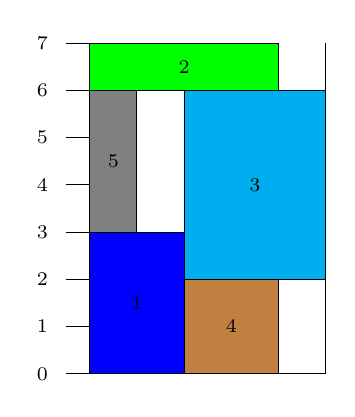
\begin{tikzpicture}[scale=0.6]
        \tikzstyle{every node} = [font=\scriptsize]
            \begin{scope}
                \foreach\x in {0,1,...,7}{
                    \draw (-0.5,\x) -- (0,\x);
                    \node at (-1,\x) {\x};
                }
               \draw (0 ,7) -- (0,0) -- (5,0) -- (5,7);
                   \filldraw[blue,draw=black] (0,0) rectangle (2,3);
                   \draw (1,1.5) node {1};

                   \filldraw[brown,draw=black] (2,0) rectangle (4,2);
                   \draw (3,1) node {4};

                   \filldraw[cyan,draw=black] (2,2) rectangle (5,6);
                   \draw (3.5,4) node {3};

                   \filldraw[gray,draw=black] (0,3) rectangle (1,6);
                   \draw (0.5,4.5) node {5};

                   \filldraw[green,draw=black] (0,6) rectangle (4,7);
                   \draw (2,6.5) node {2};

             \end{scope}
         \end{tikzpicture}
        \caption{Simple example}
    \end{figure}
\end{frame}



\section{State of Art}
\label{stateofart}
Today, there are numerous papers around the strip-packing problem,
due the widely situations which this problem can be applied.
We consider some related publications to perform a general review
of the solution for this problem, including the most representative
meta-heuristics, and heuristics methods.

A good review of some representative solutions can be found in the work
presented in \cite{hooper}, considering meta-heuristics and search heuristics,
but also describe the most representative placement heuristics,
which is an important aspect in a contruction of any solution,
because it is possible to use a sofisticated meta-heuristic,
but if is incompatible with the placement mechanism,
could return inefficient solutions.
Furthermore, \cite{hooper} notes some final aspects to take into account
when developing a solution, it is possible to obtain good implementation in:
\begin{itemize}
    \item Execution time, i.e. fast algorithms; (Bottom-Left)
    \item Best layout, i.e. less used area (Simulated Annealing).
    \item Good scalability, considering a similar performance with different
        problem sizes (Genetic and Naïve evolution algorithms).
\end{itemize}

Additionally the work presented by \cite{riff},
show a brief and simple analysis of some important
publications, testing the proposed implementations
and obtaining two fundamentals conclusiones:
\begin{itemize}
    \item It is important to note that when a new solution is proposed
        the benchmark to compare results, can return more efficient or
        inefficient results.
    \item Reaffirms that the implementation based on Genetic algorithms are well
        suited to obtain good solutions.
\end{itemize}

This section aims to collect some actual good approaches
to solve the strip-packing problem.

\subsection{Heuristics}

\subsubsection{Based on best-fit heuristic}

In the work presented by \cite{burke}
a new methodology was presented which modify the
way to determine the penalization of each item position.

The base methodology is find the difficult items (high penalty),
and use them first, leaving the easiest items (low penalty)
positioning, to the end of the algorithm.

The algorithm search the item positions which break bound
constraints and assign it a penalization based on the existing
penalization plus the size of the height (considering filling the space
from above).

\subsubsection{Non-guillotinable}

Several solutions in the artificial intelligence field
are based on "real-life" situations, and the work presented
by \cite{leung} is a good example.
Considering the a non-guillotinable scenario, allowing
the items rotation, a solution was propose based on
the wall-building rule (bricklaying heuristic), generating a fast algorithm
for large scale problems.

The main idea, is to initiate each layer with one item o
a set of items with the same width, leaving empty space,
which is filled up following the BL heuristic.
Finally a Greedy search is used to improve the results.



\subsection{Meta-heuristics}

\subsubsection{Non-based on bottom-left heuristic}

There are some publications which provides a very clever
approach to solve this problem.
When a researcher start to think in a new method for
solving any optimization problem, take as basis
the best results in the literature,
but in some cases, the authors think in a whole new way
to find a solution, which is the case of \cite{neveu},
that provide a method starting from one of the most critic
issues solving the problem, the blank-spaces.

In the literature is possible to find methods to avoid
this blank-spaces (holes), re-adjusting the pieces,
or adding a penalization, but this works presented the
idea of maintain a set of maximizes blank-spaces in the
process of adding new items.
The key, is that maintaining blank-spaces allows the
algorithm to not modify the entire solution when a item
is removed, reducing this algorithm cost,
which in other cases is a critical factor.

\subsection{Hyper-Heuristics}

Most of the presented solutions are based in one placement heuristic,
but in terms of Hyper-Heuristic, \cite{burke2} present a total
paradigm change considering the genetic programming methodology,
evolving heuristics instead of solutions, i.e. the genetic algorithm
will not search the place for each object, but different variations.
The implementation use heuristics based in one of the more efficient
ones, the Best-fit heuristic
In each iteration, the population of heuristics has an associated
value which determine how good it is.

\subsection{Exact methods}

One of the exact methods to solve the strip-packing problem,
is the branch and bound approach,
which only consider solutions using all the necessary items
to fill the entire space.
The idea behind this approach, is solve the situations when
is not possible to add a new item in the space,
without generate an empty space (hole),
so the algorithm start to cut branches.

In the presented work by \cite{alvarez},
the focus is over add new conditions to the strips,
to be able to generate better solutions,
also reduces the problem to different knapsack problems using the slides,
before apply the lower bounds.
Almost all the main ideas of the implementations,
are based on the work presented by \cite{martello},
chiefly the idea of use computed lower bound,
relaxing some constraints of the items surface,
dividing each item in slides to search solutions
more easily, but also considering that at the end of the algorithm,
is essential to join all the slides of the different items.


% "A branch and bound algorithm for the strip packing problem"
% 
% - Desarrollan lower bounds basados in formuationes de relajaciones enteras
% - Basan la mayoria del algoritmo (structure of the search tree) de Martello et al 2003
% - Proponen nuevas lower bounds
% - Primer se aplica la reducción (utilizan GRASP para ver si las piezas caben en un rectangulo)
% - Despues terminan las tiras y piezas para resolver un problema de la mochila (knapsack)




\section{Conclusions and Future Work}
\label{conclusions}
We presented  a brief review for the two-dimensional strip-packing
considering different approaches to obtain an optimized solution.

The idea of the next work is improve and expand this current review,
and propose a new method, using the best ideas of the literature
focused on solving the presented problem.


%\bibliographystyle{splncs03}
%\bibliography{report}

\end{document}
